


\chapter[Quantum orbits as trajectories through complex time and complex\texorpdfstring{\\}{} space]{Quantum orbits as trajectories through complex time and complex space}
\label{chap:quantum-orbits}
\chaptermark{Quantum orbits as trajectories through complex time and complex space}

This chapter examines in closer detail the structure of the complex-valued electron trajectories used by the Analytical $R$-Matrix theory of photoionization: where it comes from, what the complex-valuedness means, how it interacts with the correlation interaction and the mean-field Coulomb potentials, under what circumstances the imaginary part becomes problematic, and how it should be handled in those conditions. 

We have built, in chapter~\ref{chap:R-matrix}, the framework for a semiclassical, trajectory-based theory of photoionization including the Coulomb and correlation interaction potential, building from the Schrödinger equation to obtainthe laser-driven trajectory
\begin{equation}
\rl(t) = \int_{\ts}^{t} \left[\vbp+\vba(\tau) \right] \: \d\tau
\label{e5-laser-driven-trajectory}
\end{equation}
as a fundamental object, and we have examined  the correlation interaction potentials that should be evaluated at this trajectory -- the reduction of the geometrical integrals to single evaluations of the potential in chapter~\ref{chap:multi-channel} and the properties of realistic and model molecular correlation interaction potentials when taken over complex coordinates in chapter~\ref{chap:complex-space-potentials}. Now we turn to the detailed properties of the laser-driven trajectory \eqref{e5-laser-driven-trajectory}.




The material in this chapter has appeared previously in reference
\begin{enumerate}
\item[{\hypersetup{citecolor=black}\citealp{Pisanty_slalom_2016}}.]
\textsc{E.~Pisanty and M.~Ivanov}.
\newblock Slalom in complex time:\ emergence of low-energy structures in tunnel
  ionization via complex time contours.
\newblock \href{http://dx.doi.org/10.1103/PhysRevA.93.043408}{
          \emph{Phys. Rev. A} \textbf{93} no.~4, p.~043\,408 (2016)}.
\newblock \href{http://arxiv.org/abs/1507.00011}{{arXiv}:1507.00011}.
\end{enumerate}
%
%
This chapter also describes work that is implemented in the software packages
\begin{enumerate}
\item[{\hypersetup{citecolor=black}\citealp{ARMSupport}}.]
\textsc{E.~Pisanty}.
\newblock {ARMSupport}: {A} support suite for {A}nalytical {$R$}-{M}atrix
  calculations.
\newblock \url{https://github.com/episanty/ARMSupport} (2016).

%\item[{\hypersetup{citecolor=black}\citealp{EPToolbox}}.]
%\textsc{E.~Pisanty}.
%\newblock {EPToolbox}.
%\newblock \url{https://github.com/episanty/EPToolbox} (2016).

\item[{\hypersetup{citecolor=black}\citealp{QuODD}}.]
\textsc{E.~Pisanty}.
\newblock {QuODD}: Quantum Orbits Dynamic Dashboard.
\newblock \url{https://github.com/episanty/QuODD} (2015).
\end{enumerate}


\vfill



\section[Emergence of complex-valued trajectories in Analytical R-Matrix theory]{Emergence of complex-valued trajectories in Analytical $R$-Matrix theory}
\label{sec:emergence-of-complex-trajectories}

Before we go into the detailed structure of the laser-driven trajectory \eqref{e5-laser-driven-trajectory}, it is important to reconstruct where exactly it comes from, and why the Analytical $R$-Matrix (ARM) theory uses this specific form as opposed to other alternatives. As we saw in the Introduction, the traditional Strong-Field Approximation (SFA) methods tend to produce ionization yields of the form
\begin{equation}
a(\vb{p})
\sim
\exp(-i\left(
 -I_{p} \ts + \frac{1}{2} \int_{\ts}^{T}\left(\vbp+\vba(\tau)\right)^2\d\tau 
\right))
,
\label{e5-sfa-like-yield}
\end{equation}
where $\ts$ is a saddle point time obeying an equation of the form $\frac12 (\vbp+\vba(\ts))^2+I_p = 0$, and this admits a natural trajectory interpretation because the Volkov phase,
\begin{equation}
\exp(-iS_V)
=
\exp(- \frac{i}{2} \int_{\ts}^{T}\left(\vbp+\vba(\tau)\right)^2\d\tau )
=
\exp(-i\int_{\ts}^{T}\frac{\vbv(\tau)^2}{2} \d\tau )
,
\label{e5-volkov-phase-for-trajectories}
\end{equation}
is exactly the semiclassical kinetic phase of a particle with velocity $\vbv(t) =\vbp +\vba(t)$, exactly that of a free electron driven by the laser field.

The problem with that is the word `free': the Strong-Field Approximation neglects effects caused by the Coulomb field, which causes it to miss several important physical effects and features of real-world spectra, so the problem to be solved is the reintroduction of Coulomb effects within this formalism, looking for a trajectory-based semiclassical theory that includes the effects of this potential.

As we saw in the Introduction, a class of methods known generally as the Coulomb-corrected Strong Field Approximation (CCSFA)~\cite{CCSFA_initial_short, CCSFA_initial_full} accomplishes this by keeping the form of the result -- $a(\vbp)\sim e^{-iS}$ -- and replacing the action by the full Coulomb action (kinetic terms as well as the Coulomb potential energy) evaluated at a full trajectory that obeys a Newtonian equation of motion driven by the laser field and the Coulomb potential. Unfortunately, however, getting the trajectory from the equation of motion is problematic, because the trajectory formulation derived from \eqref{e5-volkov-phase-for-trajectories} says nothing about the initial condition to be used, and this needs to be supplied by~hand.


The ARM theory, on the other hand, gets its results directly from the boundary matching procedure of chapter~\ref{chap:R-matrix}, and this means that it gets its trajectory~\eqref{e5-laser-driven-trajectory}, initial conditions and all, in a traceable line from the Schrödinger equation. This has the direct advantage that the trajectory no longer includes any arbitrary components, but for this we must pay the price that the theory only uses the laser-driven trajectory instead of the full Newtonian equation of motion. 

In fact, as we shall see later, our study of the structure of~\eqref{e5-laser-driven-trajectory} shows that the ideal theory, one that builds from first principles through to the full trajectory, will likely face a number of difficulties that disappear when one has control over the initial condition, but which come naturally to the first-principles tunnelling theory. At the moment, though, the situation is roughly the one sketched in \reffig{f5-holy-grail-table}: the ideal theory, as yet unavailable and possibly outside the realm of the reasonably obtainable, should incorporate the first-principles aspects of ARM theory and the full trajectory used by CCSFA methods, but at the moment all we have are those two dual approaches to help us understand what features the ideal theory should have, what problems it will probably meet, and what tools are available to resolve those.






\begin{figure}[htb]
\centering
\begin{tabular}{>{\centering\arraybackslash}m{0.7cm}>{\centering\arraybackslash}m{9.5cm}}
$\,$&
\Large
\hspace{-7.5mm}
$\displaystyle\stackrel{\text{full action}}{\xrightarrow{\hspace*{7.5cm}}}$
\vspace{0mm}
\\  %\hline
\Large
\rotatebox{90}%
{
\hspace{-5mm}
$\displaystyle\stackrel{\text{first principles}}{\xleftarrow{\hspace*{4.2cm}}}$
\hspace{0.5mm}
}
\hspace{-50mm}
& 
\hspace{-7.5mm}
\begin{tabular}{|>{\centering\arraybackslash}m{1cm}|>{\centering\arraybackslash}m{7.3cm}|}
\hline
\vspace{2.5mm}  SFA   \vspace{1.5mm}  & 
\vspace{2.5mm} CCSFA \vspace{1.5mm}  \\ \hline
ARM & 
\vspace{4mm}  
\includegraphics[height=4cm]{5-Quantum-orbits/Figures/figure5A.png}  \hspace{-1mm}\vspace{3mm}
\\ \hline
\end{tabular}
%\\ \hline
\end{tabular}
\vspace{4mm}

\caption[Schematic relationship between the SFA, CCSFA and ARM theories]{
Schematic depiction of the relationship between the Strong-Field Approximation (SFA), the Coulomb-corrected Strong-Field Approximation (CCSFA), and the Analytical $R$-Matrix (ARM) theory presented here. Ideally, we would like a first-principles derivation of a semiclassical theory building on the SFA and including Coulomb effects with the full Coulomb action: ARM theory approaches on the first-principles side and CCSFA uses a full Coulomb action, and both illuminate important aspects of the ideal theory.
}
\label{f5-holy-grail-table}
\end{figure}
\copyrightfootnote{
Holy Grail image in \reffig{f5-holy-grail-table} excerpted from \textit{Monty Python and the Holy Grail}, © National Film Trustee Company Ltd, 1974.
}




For now, though, we focus on the task at hand and examine the origin of the ARM trajectory \eqref{e5-laser-driven-trajectory}. The ARM gets its trajectory language, ultimately, from the same place that the usual SFA does: from its continuum wavefunctions. However, while the SFA takes its kinetic phase from the Volkov states
\begin{align}
\phantom{{}^\mathrm{EA}}
\braket{\vb{r}}{\vb{k}^{\mathrm{(V)}}(t)}
& = 
\frac{1}{(2\pi)^{3/2}}
e^{i\left(\vb{k}+\vba(t)\right)\cdot\vb{r}} 
e^{-\frac{i}{2} \int_T^t\left(\vb{k}+\vba(\tau)\right)^2\d\tau}
,
\phantom{e^{-i\int_T^t U_n(\rl(\tau;\vb{r},\vb{k},t),\tau)\d\tau}}
\backtag{e2-volkov-wavefunctions}
\end{align}
in ARM theory we introduce the Coulomb correction at this same wavefunction level where the trajectory language starts. Thus, ARM theory introduces the Coulomb phase $e^{-iW_C}=e^{-i\int_T^t V(\rl \d\tau}$ here, giving
\begin{align}
\braket{\vb{r}}{\vb{k}^{\mathrm{(EVA)}}(t)}
& = 
\frac{1}{(2\pi)^{3/2}}
e^{i\left(\vb{k}+\vba(t)\right)\cdot\vb{r}} 
e^{-\frac{i}{2} \int_T^t\left(\vb{k}+\vba(\tau)\right)^2\d\tau} 
e^{-i\int_T^t V(\rl(\tau;\vb{r},\vb{k},t),\tau)\d\tau},
\backtag{e2-eikonal-volkov-wavefunctions}
\end{align}
in terms of laser-driven trajectory
\begin{align}
\rl(\tau;\vb{r},\vb{k},t)
& \colonequals 
\vb{r}+\int_t^\tau \left(\vb{k}+\vba(\tau')\right)\d\tau'
.
\backtag{e2-trajectory}
\end{align}
Moreover, the form of this Coulomb phase $e^{-iW_C}$, and the trajectory it builds from, are not imposed on the wavefunction. Instead, the eikonal approximation \cite{eikonalVolkov_initial, eikonalVolkov_prelim} builds this phase from a WKB-like semiclassical series, which transforms the Schrödinger equation for $e^{-iS}$ into a Hamilton-Jacobi equation in $S$, whose solutions are precisely those built over the classical trajectories.

Implementing the eikonal-Volkov wavefunctions, on the other hand, does require additional machinery, because their perturbative treatment of the Coulomb field means that they cannot get too close to the ion and its Coulomb singularity. While this is not the only reason to introduce the $R$-matrix splitting of space into inner and outer regions (which is also essential for multi-electron effects), it does make the two methods ideally suited for each other. 

This means, then, that the eikonal Volkov states need to be matched at the $R$-matrix boundary using the procedure of chapter~\ref{chap:R-matrix}, and this connects them to a similar wavefunction on the other side -- the WKB tail of the ionizing orbital, which is also essentially of~the form
\begin{equation}
\psi_g(r) \propto C_\kappa e^{-i\int_{\tk}^{\tvr}U\left(\int_{\ts}^\tau \vbv(\tau')\d\tau' \right)\d\tau}.
\label{e5-ground-state-WKB-revisited}
\end{equation}
Here the `starting' time $\tk$ has some leeway, as changing $\tk$ only changes $\psi_g$ by a constant that can be absorbed into $\tk$, but the convenient choice is to set it to $\tk=\ts-i/\kappa^2$, which permits the WKB ground state \eqref{e5-ground-state-WKB-revisited} to coincide with the explicit expression \eqref{e2-wkb-explicit-expression} for the wavefunction. In trajectory language, this choice implies that the position at $\tk$ is roughly $1/\kappa$, the characteristic distance of the ionizing orbital. (This separation, while small, is nevertheless crucial, because for a Coulomb singularity the integral in~\eqref{e5-ground-state-WKB-revisited} diverges if taken for a trajectory that starts at the origin with $\tau$ up~to~$\ts$.)

The trajectory formulation for the ionizing state's WKB expression~\eqref{e5-ground-state-WKB-revisited} is the ultimate source of the initial condition for our final laser-driven trajectory \eqref{e5-laser-driven-trajectory}, since the eikonal-Volkov states \eqref{e2-eikonal-volkov-wavefunctions} are based on trajectories \eqref{e2-trajectory}, which have an arbitrary starting point set to the evaluation point $\vbr$; these starting points are averaged over the $R$-matrix boundary in the matching procedure and reduce to the WKB expression with a trajectory that starts at the origin at the ionization time~$\ts$.




%
%\subsection{Overview}
%Finally, and before we begin the technical analysis in earnest, it is worthwhile to comment on the lay of the land ahead. 
%
%
%
%
%





\section{Imaginary parts of the laser-driven trajectory}
Having examined the pedigree of our laser-driven trajectory, 
\begin{equation}
\rl(t) = \int_{\ts}^{t} \left[\vbp+\vba(\tau) \right] \: \d\tau
,
\backtag{e5-laser-driven-trajectory}
\end{equation}
we now turn to its structure. We focus specifically on a monochromatic field of the~form
\begin{equation}
\vba(t)=-\frac{F}{\omega}\un \sin(\omega t),
\backtag{e2-field-definition}
\end{equation}
though most of the results that follow will degrade smoothly if a reasonably slow envelope is introduced. In this chapter we will work in the laboratory frame, fixing the polarization direction to the $z$ axis.

Generally speaking, the laser-driven trajectory should be thought of as a general analytical function $\rl\colon \mathbb{C}\to \mathbb{C}^3$, and in principle it is defined for an arbitrary complex input, for which it reads
\begin{equation}
\rl(t)=(t-\ts)\vbp +\frac{F}{\omega^2}\uz \left(\cos(\omega t) - \cos(\omega \ts)\right)
,
\label{e5-explicit-rl-trajectory}
\end{equation}
with the cosine taking an arbitrary complex input as usual.

More specifically, though, we care about $\rl(t)$ because we need it to calculate the temporal integrals over the mean-field Coulomb potential as 
\begin{equation}
\int_\tk^T U_n(\rl(\tau)) \d\tau
\label{e5-coulomb-rl-integral}
\end{equation}
for the single-electron yield~\eqref{e2-ionization-yield-with-shape-factor}, and 
\begin{equation}
\int_{\ts}^T\! \Vnm{\rl(t)} e^{+i(E_n-E_m)t} \: \d t 
\end{equation}
over the correlation interaction potential for the correlation-driven yield~\eqref{e3-correlation-driven-yield-reprise-with-full-derivatives}. Both of these integrals start at (or near) the complex ionization time $\ts$, and they need to be taken until the detection time $T$, which should be large enough for the pulse to be over and for all ionization effects to have converged. 

Since the integrands in both cases are analytical, the path for these integrals can in principle be chosen arbitrarily, and the integral will always evaluate to the same value. However, for the sake of definiteness, as we saw in the Introduction with \reffig{f1-initial-contour}, the convention is generally to start at the complex ionization time $\ts = \tn + i\tauT$, integrate directly down to its real part $\tn=\Re(\ts)$ on the real axis, and then along the real axis until the detection time $T$, as shown in \reffig{f5-standard-time-contour}.


\begin{figure}[htb]
\centering
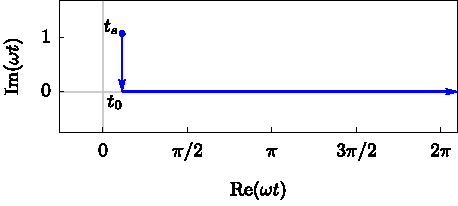
\includegraphics[scale=1]{5-Quantum-orbits/Figures/figure5B.pdf}
\caption[Standard integration path in the complex time plane, from the ionization time $t_s$ to its real part and then along the real axis]{Standard time contour used in complex-time theories of tunnelling ionization: down from the complex ionization time $\ts$ to its real part $\tn=\Re(\ts)$, and then along the real axis until the detection time $T$.}
\label{f5-standard-time-contour}
\end{figure}


This sort of contour is particularly useful conceptually, because it allows us to usefully separate a ``tunnelling'' part of the integration (the downward leg, where factors of the form $e^{-iEt}$ for complex $t$ impose the exponential unlikelihood of tunnelling processes) from a more classical propagation along the real axis where $e^{-iEt}$ factors are only phases as~usual and the electron is generally understood as having left the classically forbidden~region. As we shall see later, this standard contour can cause problems when we turn time into position using our laser-driven trajectory \eqref{e5-laser-driven-trajectory} and we run this through our potentials, but it is useful in many scenarios and it is certainly a reasonable default choice.


If we analyse this standard contour in terms of the trajectory $\rl(t)$, the most interesting part is the tunnelling segment -- the downwards leg from $\ts$ to $\tn$. Here, breaking the trajectory~\eqref{e5-explicit-rl-trajectory} down into explicit real and imaginary parts for an argument of the form $t=\tn+i\tau$, we can express it as
\begin{align}
\rl(\tn+i\tau)
= &
- i(\tauT-\tau)\vbpo
\nonumber \\ & \quad
+\frac{F}{\omega^2}\uz \left[\vphantom{\sum^n}
-\cos(\omega\tn)
\left( \vphantom{\sum}
\cosh(\omega\tauT)
-\cosh(\omega\tau)
\right)
\right. \nonumber \\ & \left. \vphantom{\sum^n} \qquad \qquad 
+i\left( 
-\omega(\tauT-\tau)\frac{\omega p_z}{F}
+
\sin(\omega\tn)(
\sinh(\omega\tauT)
-\sinh(\omega\tau)
)
\right)
\right]
.
\label{e5-explicit-rl-trajectory-re-im-parts}
\end{align}
%
Here we see that the combination $\cos(\omega t) = \cos(\omega \tn + i \omega\tau)$ will generally always produce a complex number whenever $\tn$, which is given by the explicit saddle-point equation
\begin{equation}
\omega \ts
=\omega\tn+i\omega\tauT
= \arcsin\left(
\frac{\omega}{F}\left(p_z + i \sqrt{\kappa_n^2+\pt^2}\right)
\right)
,
\backtag{e2-saddle-point-equation-final-solution}
\end{equation}
has a nonzero real part, which happens whenever $p_z$ is nonzero. Outside of the special case of $p_z=0$, then, the laser-driven trajectory $\rl(t)$ is always complex-valued once $t$ reaches the foot of the contour at the real axis, following the behaviour shown in \reffig{f5-imaginary-parts-of-position}.


\newcommand{\onemicronparsfield}{0.05} 
\newcommand{\onemicronparsomega}{0.0456} 
\newcommand{\onemicronparskappa}{1.07} 
\newcommand{\onemicronparswavelength}{1} 
\newcommand{\onemicronparsgamma}{0.98}
\begin{figure}[htb]
  \centering
  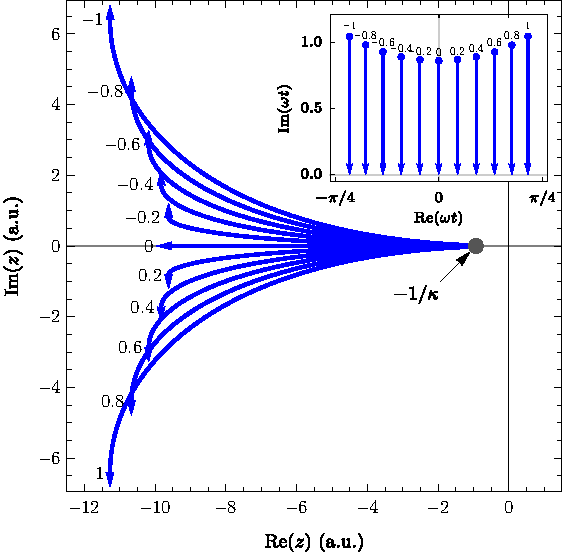
\includegraphics[scale=1]{5-Quantum-orbits/Figures/figure5C.pdf}
  \caption[
  Laser-driven trajectory $\zl(t)$ in the complex $z$ plane, over the ``tunnelling'' downwards leg of the standard time contour
  ]{
  The laser-driven trajectory $\rl(t)$ on the complex $z$ plane, corresponding to the ``tunnelling'' part of the standard contour where $t$ goes from the complex tunnelling time $\ts$ down to its real part $\tn$ on the real axis, with the time contour segments shown in the~inset.
  Here, and in the rest of this chapter unless otherwise stated, we set $F=\SI{\onemicronparsfield}{\au}$, $\omega=\SI{\onemicronparsomega}{\au}$ and $\kappa=\SI{\onemicronparskappa}{\au}$, corresponding to argon ionized by a $\SI{\onemicronparswavelength}{\micro m}$ field at $\SI{e14}{W/cm^2}$, with Keldysh parameter $\gamma=\onemicronparsgamma$.
  }
\label{f5-imaginary-parts-of-position}
\end{figure}


In addition to this, if there is any nonzero transverse momentum $\vbpo$ orthogonal to the polarization direction, then upon reaching the real axis the position on the transverse plane will be completely imaginary, at $-i\tauT\vbpo$, since here the electron has a real velocity and propagates through an imaginary time interval. 

In the longitudinal direction, on the other hand, in the special case that $p_z=0$ the electron has a completely imaginary velocity $v_z(\ts)=\sqrt{-2I_p}$, and it propagates over an imaginary time interval, so it accrues only real-valued changes in position, as it does in the quasi-static case described in the Introduction. For nonzero $p_z$, on the other hand, the velocity is only completely imaginary at the moment of tunnelling, but it acquires a nonzero real component as the electron crosses the classically forbidden region, and this results in a nonzero imaginary part that increases with $|p_z|$.

On the other hand, once the integration contour reaches the real axis, this imaginary part of $\rl(t)$ can be considered to be `frozen' as long as the time contour stays on the real axis, because the velocity $\vbp+\vba(t)$ is real-valued there so its integral can only accumulate real-valued changes. 

One approach to this is to take this as a marker that the imaginary part of the position is an artefact of the method, which is only valid as a construct for use in computations: it no longer plays a role in the dynamics of the trajectory,%
%
\footnote{%
However, it is worth pointing out that for a complex-valued trajectory under the action of the Coulomb potential this is no longer true, and the imaginary part will both change and affect the evolution of the real part. Thus, dismissing the dynamics of the imaginary part of the trajectory over the real time axis is equivalent to closing the door on extensions to the theory that include Coulomb-corrected trajectories.
}
and it only needs to be tracked as a calculational tool to compute the quantum Coulomb corrections, but one can argue that it has no physical significance. (Of course, this can be said about any given concept in a physical theory.) Even within that viewpoint, however, the imaginary part of the trajectory is operationally as relevant as the real part. Moreover, it is important to note that complex-valued trajectories are not confined to this method, and they are a rather general feature of quantum mechanics when it is pushed into trajectory language~\cite{goldfarb-tannor_bohmian-complex_2006, goldfarb-tannor_complex-trajectory-wkb_2008, schiff-tannor_path-integral-complex-trajectory_2011}. 

In addition, connecting back to our motivations for finding trajectory language in the first place, we set out to see if it is possible to derive a model, entirely within the TDSE and without adding in the Coulomb field by hand, that includes the trajectory language used by CTMC approaches. The ARM results then teach us that it is indeed possible, but that the TDSE-based trajectories come with a complex component, and that one ignores this at one's own peril. With this we turn, then, to the consequences of this imaginary part when it is included in the Coulomb interaction.











\section{Emergence of temporal branch cuts}
As we saw in chapter~\ref{chap:complex-space-potentials}, in general it is possible to calculate the correlation interaction potential $\Vnm{\rl(t)}$ when the argument $\vbr=\rl(t)$ is complex, but this needs to be confined to the safe region
\begin{equation}
\Re(\vbr^2)>0
\backtag{e4-re-r2-less-than-0}
\end{equation}
where the gaussian-based methods give reasonable answers and we can be reasonably sure that our models are correct, so we need to ensure that the laser-driven trajectory never leaves this region.

In addition to this, the mean-field potential $U_n(\vbr)$ also imposes requirements when it is applied to a complex argument. These requirements can be similar to those of the correlation interaction potential when $U_n(\vbr)$ is taken to be the mean field of a full molecular charge, but in this chapter we will focus on the bare basics of this potential and simply take it to be a Coulomb potential, which is in any case always present. This will be plenty to keep us busy, and most of the results generalize to a broader class of potentials.

The Coulomb potential is problematic because, when extended to its analytical continuation over complex positions, it requires a square root to remain analytical:
\begin{equation}
U(\vbr) = -\frac{1}{\sqrt{\vbr^2}}= -\frac{1}{\sqrt{x^2+y^2+z^2}}.
\label{e5-coulomb-potential}
\end{equation}
This means that the Coulomb potential goes from having an integrable singularity at the origin to having a branch cut along the ray $\vbr^2\in (-\infty,0]$; this is where the standard branch, as we defined it in \eqref{e4-square-root-definition}, resolves the ambiguity of whether to assign $\sqrt{-1}$ to $+i$ or $-i$ by having a discontinuous sign change of the imaginary part: numbers with a slightly positive imaginary part are assigned to the neighbourhood of $+i$, as $\sqrt{-1+i\varepsilon}\approx i+\varepsilon/2$, and numbers with a slightly negative imaginary part are assigned to the neighbourhood of $-i$, as $\sqrt{-1-i\varepsilon}\approx -i+\varepsilon/2$.



However, unlike our previous encounter with this branch cut in \eqref{e4-square-root-definition}, where all we needed was a definite integrand to calculate with, here the Coulomb cut has very deep consequences, because the Coulomb potential is now being directly integrated in a complex path integral. Indeed, if one integrates across the branch cut's discontinuity, the dependence on $t$ of the Coulomb integrand in \eqref{e5-coulomb-rl-integral} ceases to be analytic, and one loses the freedom that allowed the real contour of \eqref{e2-yield-after-saddle-point-approximation} to be deformed to pass through the saddle-point $\ts$ in the first place. In other words, all the work since the initial saddle-point approximation over the tunnelling time $\ts$ would become invalid.



\captionsetup[figure]{position=auto}

\begin{figure}[t!]
  \centering
  \captionsetup[figure]{position=b}
  \captionsetup[subfigure]{position=b}
  \subfloat{
    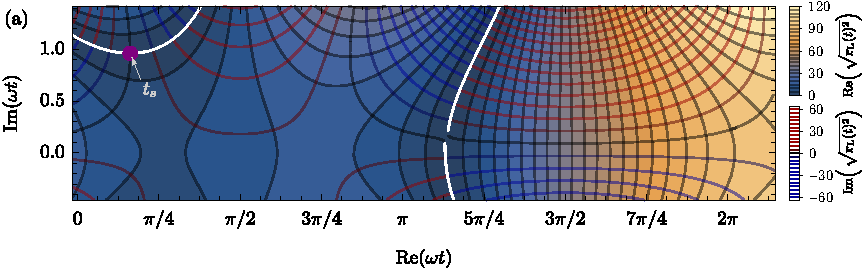
\includegraphics[scale=1]{5-Quantum-orbits/Figures/figure5Da.pdf}
    \label{f5-complex-position-contour-plot}
  }
  \\[-3mm]
  \subfloat{
    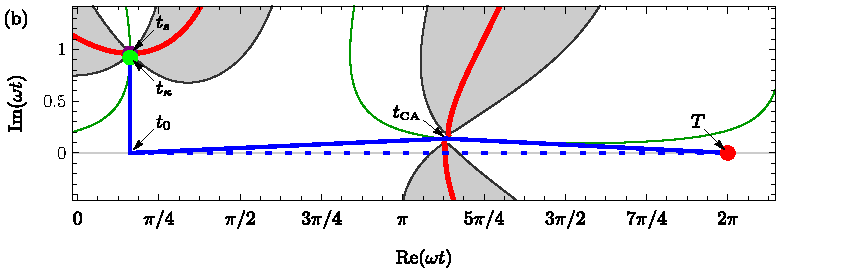
\includegraphics[scale=1]{5-Quantum-orbits/Figures/figure5Db.pdf}
    \label{f5-branch-cut-sketch}
  }
  \captionsetup{width=\textwidth}
  \caption[
  Riemann surface of $\sqrt{\rcl(t)^2}$ over the complex time plane, showing branch cuts that cross the standard integration path along the real axis
  ]{
  \protect\subref{f5-complex-position-contour-plot} Contour plot of the complex distance to the origin, $\sqrt{\rcl(t)^2}$, with the coloured background along the real part and the red, black and blue orthogonal lines representing, respectively, positive, zero and negative imaginary parts. The white lines are branch cuts where the real part is zero and the imaginary part discontinuously changes sign.
  In \protect\subref{f5-branch-cut-sketch} we show a simplification of this picture, with the red lines showing the branch cuts, and the thin green lines the positive real axis of $\vbr^2$. The shaded regions indicate the complex times for which $\Re(\rcl(t)^2)$ is negative, which are undesirable when using gaussian and numerically-obtained ionic potentials, as they would be unphysical there.
  The momentum displayed, $\vbp=(\figurefiveDpo,0,\figurefiveDpp)$, is such that the standard contour (integrating down to the real part $\tn$ of the saddle point $\ts$ and then along the real axis, shown dotted in \protect\subref{f5-branch-cut-sketch}) crosses a branch cut. Instead, one should choose a contour which passes through a time between the branch cuts, which we label $\tca$ and explore in detail in Sec.~\ref{sec:times-of-closest-approach}.
  }
  \label{f5-complex-position-branch-cuts}
\end{figure}


To be somewhat more definite, the branch cut occurs when $\vbr^2$ is real and negative, and~since we can write it as
\begin{equation}
\vbr^2=\Re(\vbr)^2-\Im(\vbr)^2+2i\Re(\vbr)\cdot\Im(\vbr),
\label{e5-r2-parts-breakdown}
\end{equation}
this means that the branch cut requires $\Re(\vbr)$ to be smaller than $\Im(\vbr)$ and occurs when the two are perpendicular. This is relatively hard to picture geometrically, but fortunately there are simpler tools to analyse this. In particular, we only need to consider the entire potential as a single, function of time,
\begin{equation}
U(\rl(t)) = -\frac{1}{\sqrt{\rl(t)^2}},
\label{e5-coulomb-potential-at-the-trajectory}
\end{equation}
a single analytical function of the complex-valued variable $t$, and in this perspective the branch cuts in $U$ are imprinted on the complex time plane via the conformal mapping $t\mapsto \rl(t)^2$. To see this, we show in \reffig{f5-complex-position-contour-plot} an example of the Coulomb potential's behaviour, as a complex conformal map of the function $\sqrt{\rl(t)^2}$ (which has the same branch-cut structure as $U$, but omits the latter's singularities). 




The essential features of this function are the branch cuts, which are shown in white, with a discontinuous sign change in the imaginary part of $\sqrt{\rl(t)^2}$. Unfortunately, the full conformal map can obscure some information, like the position of the real axis, so we show in \ref{f5-branch-cut-sketch} a sketch with the essentials of this function, with the branch cuts shown in red. Here it is important to note that the standard integration contour of \reffig{f5-standard-time-contour} -- straight down from the complex ionization time $\ts$, and then along the real axis, shown dotted in \reffig{f5-branch-cut-sketch} -- can indeed cross the branch cuts when the electron returns near the ion.



\begin{figure}[t!]
  \centering
  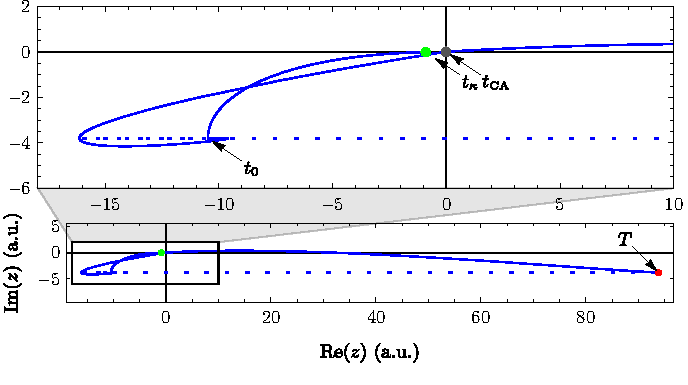
\includegraphics[scale=1]{5-Quantum-orbits/Figures/figure5E.pdf}
  \caption[
  Complex-space trajectory $\zcl(t)$ corresponding to an integration path altered to avoid a Coulomb branch cut
  ]{
  Trajectories in the complex $z$ plane corresponding to the contours shown in \reffig{f5-branch-cut-sketch}. The trajectory starts at $z=-1/\kappa$ at time $\tk$, and departs somewhat from the real position axis as the time goes down to the real axis at $\tn$, as shown in \reffig{f5-imaginary-parts-of-position}. Along the real axis, on the standard contour shown dashed, the electron goes to large negative $\Re(z)$ before turning around towards the core. It then reaches the ion with a large imaginary part, which causes a discontinuous jump in the square root of~\eqref{e5-coulomb-potential}. Deforming the contours to avoid the branch cuts, shown in the solid line, minimizes the imaginary part of $z$ at the moment of recollision; it is then slowly regained before detection at a large real time $T$. The closest approach time $\tca$ marks the minimum value of $\Re(\rcl(t)^2)$ once the $x$ coordinate is taken into account; there $\zcl$ is small but nonzero.
  }
  \label{f5-complex-z-curved-contours}
\end{figure}



This means that to preserve the analyticity of the Coulomb integral~\eqref{e5-coulomb-rl-integral} one must deform the integration contour away from the real axis until the integrand is continuous and analytic throughout the integration path. This will correspondingly change the way the complex position $\rl(t)$ moves through complex space, and the effect turns out to be one of \textit{minimizing} the imaginary part of the position at the time of recollision, when $\Re(\vbr)$ is small, so that the branch cut from \eqref{e5-r2-parts-breakdown} is then avoided. We show in \reffig{f5-complex-z-curved-contours} the corresponding change in the path of $\zl(t)=\uz\cdot\rl(t)$ through the complex plane, as the time $t$ traces out the original, standard time integration contour, shown dashed, and the new, modified contour that avoids the branch cuts, shown as a solid line.


The relationship between the chosen temporal contour and the corresponding trajectory in complex position space, particularly along $z$, is in general rather complicated and it is a hard quantity to visualize. Similarly, the final momentum $\vbp$ has a strong effect on the dependence of the potential $U(\rl(t))$ as a function of time, sometimes very sensitively. To complicate matters further, these variables are all intertwined, with the changes in the momentum affecting the structure of the branch cuts, and therefore the possible paths that the time integration contour can take.



The intertwining of these variables makes the analysis of these situations relatively awkward, and to help disentangle these effects the author has written a software package, the Quantum Orbits Dynamic Dashboard software available as \citer{QuODD}, that enables the user to visualize the effects on the complex-space trajectory of different modifications on the complex-time integration path and of changes in the momentum or the ionization time~$\ts$. We display, in \reffig{f5-quodd-screenshot}, a screen capture of this software, along with its major features. Among other features, the package allows the wide variety of different integration paths to be visualized, by showing in real time the effects of such modifications on the complex-space trajectories as well as the Coulomb integrand.




\begin{figure}[htb]
  \centering
  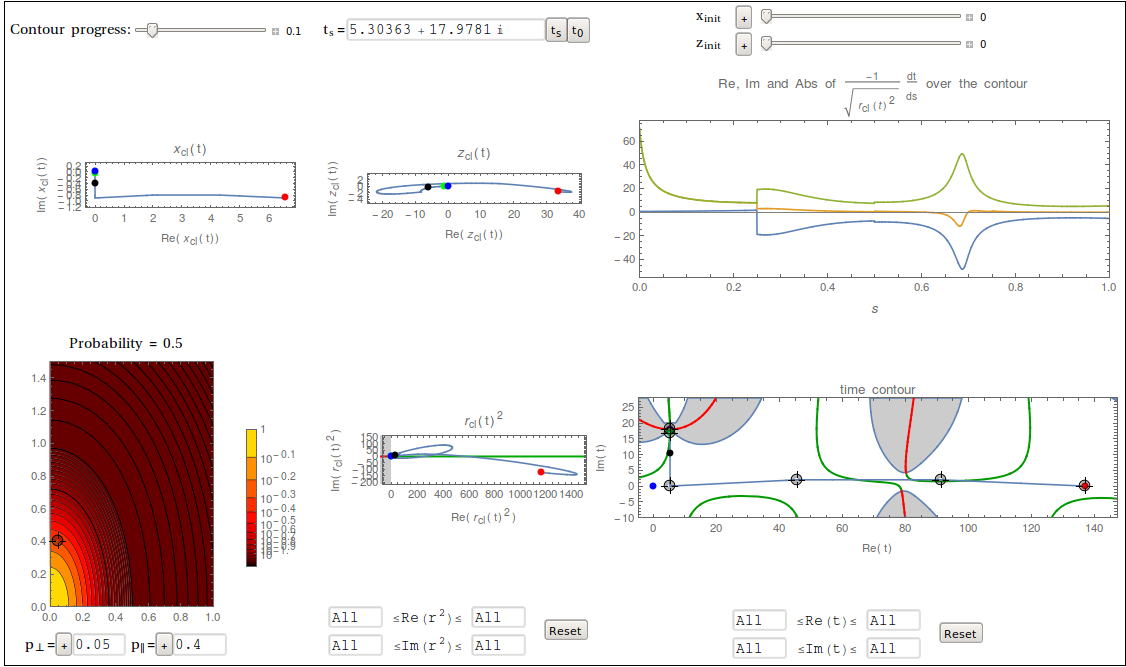
\includegraphics[width=\textwidth]{5-Quantum-orbits/Figures/figure5M.png}
  \captionsetup{width=\textwidth}
  \caption[
  Screenshot of the Quantum Orbits Dynamic Dashboard software
  ]{
  Screenshot of the Quantum Orbits Dynamic Dashboard software from \citer{QuODD}, an open-sourced Mathematica package. The main panels show, on the top row, the $x$ and $z$ coordinates of the laser-driven trajectory, together with the Coulomb integrand, for an integration path over complex time shown at bottom right over a branch cut sketch similar to \reffig{f5-branch-cut-sketch}. (Similarly, the bottom-centre panel shows a complex-plane plot of $\rl(t)^2$.) This integration path, along with the asymptotic momentum $\vbp$, shown at bottom left, and the ionization time $\ts$, can be dynamically modified, with the effects of these modifications on the trajectory and the branch-cut layout tracked in real time.
  }
\label{f5-quodd-screenshot}
\end{figure}






The presence of these Coulomb branch cuts in the complex plane has appeared in the literature occasionally~\cite{popruzhenko_branch-cuts_2014}, but only rarely has it been necessary to shift the integration path away from the sandard contour~\cite{ popruzhenko_branch-cuts_2014, Milosevic_scattering_large}. However, as we have shown, once the electron trajectory is obtained from the ground state through the ARM boundary matching, instead of having an initial condition imposed externally, they become inevitable.

In the rest of this chapter we will show how to handle these branch cuts, by providing an algorithm to programmatically choose a correct integration path, and we will explore the rich geometry unearthed by its key constituents, the times of closest approach to the ion. Later on, in chapter~\ref{chap:LES-NZES}, we will use this method to relate our calculations to experimental features photoelectron spectra. 

A more recent analysis~\cite{keil_branch-cuts_2016}, focusing on ATI spectra at the crossover between direct and rescattered electrons at $2U_p$, also confirms our findings, showing that the photoelectron spectrum there can only be analyzed correctly if a complex tunnel exit is taken into account, with the attendant branch cuts similarly forcing changes in the integration path, which can again be handled well with the method that we provide below.












\section{Times of closest approach}
\label{sec:times-of-closest-approach}
We see, then, that it is possible for branch cuts of the Coulomb potential to cross the real axis, thereby precluding the use of the standard integration contour of \reffig{f5-standard-time-contour} for the Coulomb integral in \eqref{e5-coulomb-rl-integral}, but that it is still perfectly possible to choose temporal integration paths which remain valid by avoiding the branch cuts, passing through the ``slalom gate'' left by the branch cuts of $U(\rl(t))$ as in \reffig{f5-complex-position-contour-plot}.

This can easily be done by hand, by shifting the contour appropriately, if only a single or a few momenta need to be handled, but it is certainly infeasible if one needs to compute a photoelectron spectrum, sampling a large number of different momenta. What is needed, then, is a computational approach: we require a programmatic way to automatically choose the correct integration contour for any given momentum.

The key to obtaining this approach is to examine in detail the space between the two branch cuts, as shown in \reffig{f5-tCA-zoom}. Each branch cut is a contour of constant $\Re(\sqrt{\rl(t)^2})$, which measn that the neighbouring contours must closely follow its direction, and circle around it when it terminates at the branch point. 

\begin{figure}[htb]
  \centering
  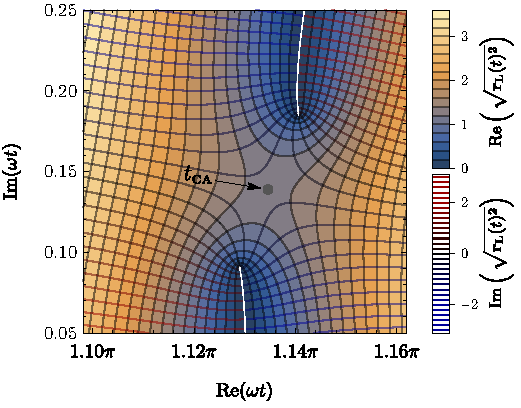
\includegraphics[scale=1]{5-Quantum-orbits/Figures/figure5F.pdf}
  \caption[
  Closer view of the `slalom gate' between two paired Coulomb branch cuts
  ]{
  Closer view of the region between the branch cuts in \reffig{f5-complex-position-contour-plot}. The space between any two branch cuts always contains a saddle point $\tca$, as this is the only way to join the curvatures of the contours next to each branch cut. For contours that pass through it, the saddle point marks the minimum of $\Re\left(\sqrt{\rl(t)^2}\right)$. For valid contours that do not pass through $\tca$, this minimum will be smaller.
  }
  \label{f5-tCA-zoom}
\end{figure}

In the slalom-gate configuration of \reffig{f5-complex-position-contour-plot}, the branch cuts come in pairs that face each other, and they must therefore have two sets of curved  contours at $\Re(\sqrt{\rl(t)^2})=\mathrm{const.}$, facing each other, that must somehow meet in the middle; the only way for this to happen is for there to be a saddle point between the branch cuts. This saddle point is the crucial object which enables the programmatic choice of a contour that avoids the branch cuts, since the saddle point is at the ideal location in between the two cuts. Moreover, the saddle point has a deep physical and geometrical significance, which we will now explore.

To begin with, it is clear from \reffig{f5-tCA-zoom} that if we track the real part of the complex distance to the origin, $\Re(\sqrt{\rl(t)^2})$, over any integration path which crosses the complex~$t$ plane from left to right of the region shown in the figure, $\Re(\sqrt{\rl(t)^2})$ must always decrease, reach a minimum, and then increase again. For some paths -- the ones that cross the branch cuts -- the minimum value of $\Re(\sqrt{\rl(t)^2})$ is zero, but these are forbidden as integration paths. From within the allowed paths, the minimum is shallowest when the path passes through our saddle point.

For this reason, then, we call the saddle point the time of closest approach, and we label it $\tca$. To be precise, then, an integration path that passes through $t=\tca$ maximizes the minimum value of the real part of the distance to the origin, $\Re(\sqrt{\rl(t)^2})$; in addition, it can also be seen to maximize the minimum value of the absolute value, $\left|\sqrt{\rl(t)^2}\right|$, as well. Intuitively, it permits the furthest possible approach to the ion, keeping the origin at arm's length as much as possible.

Similarly, when calculating the Coulomb potential along such a contour, this choice of path minimizes the maximum value of the real part and absolute value of $1/\sqrt{\rl(t)^2}$ (for valid contours which do not cross the branch cuts), so that the Coulomb interaction is kept as bounded as possible throughout the integration. As long as the potential $U(\rl(t))$ stays continuous and analytic, this is not essential (as the integral in \eqref{e5-coulomb-rl-integral} will not change) but passing through $\tca$ means reaching a smallish value through adding smallish quantities, rather than through cancellations between bigger ones. In addition, this choice optimizes the applicability of the approximations that led to \eqref{e5-coulomb-rl-integral}, and it admits the clearest physical interpretation by keeping the imaginary part of the position within the tightest relevant bound possible at the points where this is necessary.

To actually find these saddle points, one simply looks for the zeroes of the time derivative of $\sqrt{\rl(t)^2}$. More simply, though, this can be reduced to the zeroes of $\tfrac{\d}{\d t}\left[\rcl(t)^2\right]$, since they coincide with the zeroes of the square root, so the main criterion is simply
\begin{equation}
\rl(\tca)\cdot\vbv(\tca)=0.
\label{e5-tca-equation}
\end{equation}
This equation is deceptively simple, and one must remember that the left-hand side is a complex-valued function of time through Eq.~\eqref{e5-laser-driven-trajectory}. Nevertheless, it has a compelling physical interpretation, for if a classical electron passes near the nucleus then it is closest to the origin when its velocity and its position vector are orthogonal. This then lends further support to our choice of name for the $\tca$.

In this spirit, then, it is worthwhile to investigate the classical solutions of \eqref{e5-tca-equation} before exploring the solutions in the complex quantum domain. As we shall see, both domains exhibit rich geometrical structures which are closely related to one another. After exploring the geometrical implications in both contexts, we shall use this knowledge to automatically generate correct integration paths for any momentum.







\subsection{Classical solutions}
\label{sec:classical-tcas}

In this context, we can introduce a classical equivalent of our theory by simply taking the real part of our working laser-driven trajectory, as
\begin{equation}
\rcl(t) = \Re\left(\int_{\ts}^{t} \vbp+\vba(\tau) \: \d\tau\right)
,
\label{e5-classical-trajectory}
\end{equation}
and only considering real times. This simplified model is widely used as the classical version of tunnelling, since it is capable of encapsulating much of the tunnelling dynamics in terms of the tunnel exit position $\rl(\tn)$ after integration over the downward leg of the standard contour, while still having a real-valued trajectory that lends itself to further manipulation, as
\begin{equation}
\rcl(t) =  \Re\left(\rl(\tn)\right) + \int_{\tn}^{t} \left[ \vbp+\vba(\tau) \right] \: \d\tau
.
\label{e5-explicit-classical-trajectory}
\end{equation}
Indeed, this real-valued trajectory is the starting point for classical-trajectory based theories like CCFSA or Classical Trajectory Monte Carlo methods, which keep the initial term $\Re(\rl(\tn))$, and then modify the subsequent continuum dynamics.

Within this model, then, the closest-approach points obey the real part of our initial equation \eqref{e5-tca-equation}, 
\begin{equation}
\Re\left[\rl(\tcacl)\cdot\vbv(\tcacl)\right]
=
\rcl(\tcacl)\cdot\vbv(\tcacl)=0
,
\label{e5-tca-classical-equation}
\end{equation}
taken over real times. Unfortunately, this equation -- like the full quantum equation~\eqref{e5-tca-equation}~-- has more solutions than the closest-approach times we want, and these are not always distinguishable from the desired $\tca$. Specifically, the turning points of the classical trajectory, away from the core, are also solutions of \eqref{e5-tca-classical-equation}, since they are also extrema of~$\vbr^2$. On the quantum side, the surface of \reffig{f5-complex-position-contour-plot} also contains saddle points at $\omega t\approx \pi/4$ and $\omega t \approx 3\pi/4$, which correspond to the turning points shown in \reffig{f5-complex-z-curved-contours} to the right and left of the position at $\tn$, respectively.  This means that, to be able to use the closest-approach times as an effective tool to avoid the branch cuts, we will need to distinguish the crucial mid-gate $\tca$ points from the other solutions, and in general this will not be trivial.

In certain cases, though, this is easy, such as for the on-axis case when $\pt=0$, where \eqref{e5-tca-classical-equation} reads
\begin{equation}
\Re\left(\zl(\tcacl)\right)v_z(\tcacl)=0
,
\label{e5-tca-classical-equation-on-axis}
\end{equation}
with solutions that separate cleanly into turning points, for which $v_z(\tcacl)=0$, and closest approaches which degenerate to nucleus flybys at $\zcl(\tcacl)=0$, as shown in \reffig{f5-classical-tca-on-axis}. In this case, the turning points can additionally be classified as minima and maxima of $\rcl(t)^2$, shown respectively in green and red in \reffig{f5-classical-tca-on-axis}, by evaluating the sign of $\tfrac{\d^2}{\d t^2}\rcl(t)^2$. At nonzero $\pt$, it is the collisions that will turn into useful closest-approach times.



\begin{figure}[t!h]
\centering
%\begin{tabular}{c}
%\raisebox{25mm}{\subfloat[]{\makebox[5mm][0mm]{} }}\hspace{-11mm} &
%\addtocounter{subfigure}{-1}
  \subfloat{
    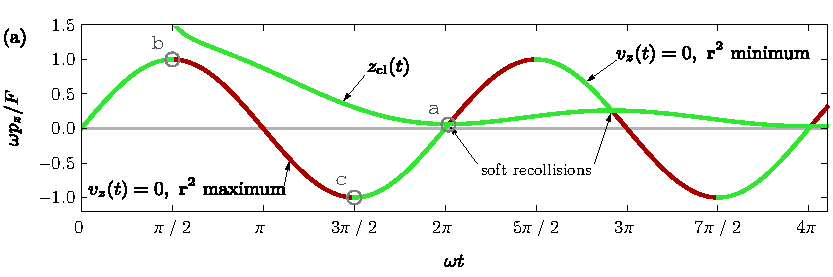
\includegraphics[scale=1]{5-Quantum-orbits/Figures/figure5Ga.pdf}
    \label{f5-classical-tca-on-axis}
  }
  \\
%\raisebox{40mm}{\subfloat[]{\makebox[5mm][0mm]{} }}\hspace{-4mm} &
%\addtocounter{subfigure}{-1}
  \subfloat{
    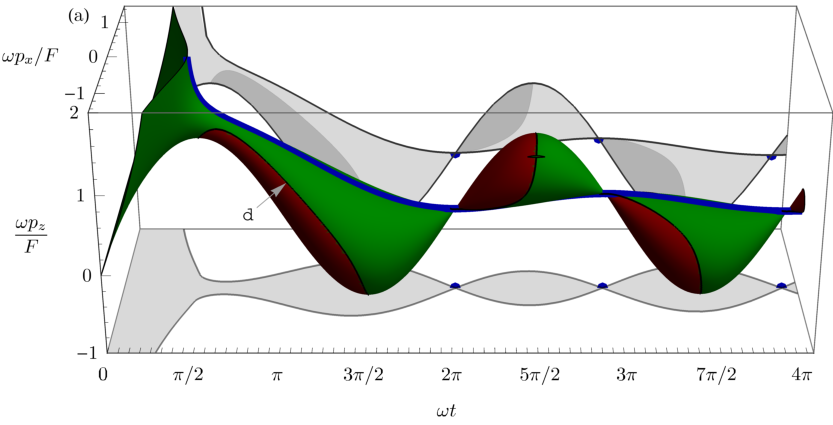
\includegraphics[scale=1]{5-Quantum-orbits/Figures/figure5Gb.pdf}
    \label{f5-classical-tca-surface}
  }
%\end{tabular}
  \caption[
  Classical closest-approach times, both on-axis at $p_\perp=0$ and as a cusped surface in $\{(\vbp,t)\}$ space
  ]{
  The classical closest-approach times with $p_\perp=0$, satisfying \eqref{e5-tca-classical-equation-on-axis}, separate into two curves  \protect\subref{f5-classical-tca-on-axis}: turning points with $v_z=0$, and collisions with $\zcl=0$, with their intersections representing soft recollisions. At the points marked \texttt{a}, \texttt{b} and \texttt{c} the different roots merge and disappear, with the corresponding trajectories displayed in \reffig{f5-sample-trajectories}.
  For nonzero $p_\perp$, the solutions of the vector equation \eqref{e5-tca-classical-equation} form a single coherent surface \protect\subref{f5-classical-tca-surface} with a sequence of bounded lobes which connect at the soft recollisions, where the surface is locally a cone.
  Local minima and maxima of $\rcl(t)^2$ are shown respectively in green and red in both panels. At the boundary between the two, a maximum and minimum meet, merge and disappear, as shown in the trajectory of \reffig{f5-sample-trajectories-d}; the point then leaves the surface.
  The side  and bottom panels show the projections of the surface on $p_z$ and $p_x$ respectively. 
  An interactive 3D version of this figure is available as Fig.~\href{https://electrondynamicsincomplextimeandspace.github.io/\#figure-s1}{S1} in the Supplementary Information \cite{SupplementaryInformation}.
 }
  \label{f5-classical-tca-plots}
\end{figure}

One of the most interesting features of \reffig{f5-classical-tca-on-axis} is the intersections of the two curves shown, the points at which $\zcl(t)=0$ as well as $v_z(t)=0$, which we will term \textit{soft recollisions} for obvious reasons. In chapter~\ref{chap:LES-NZES} we will link these soft recollisions to interesting physical effects and features on the photoelectron spectra, but for now we will focus on their pivotal role within the geometry of the times of closest approach. Even in the restricted geometry of \reffig{f5-classical-tca-on-axis} they are already crucial, since at these points the number of available roots as $p_z$ is swept across them changes from one to three, as an `inward' turning point turns into an `outward' turning point flanked by two closest-approach points. The classical trajectory shows exactly this behaviour, as shown in \reffig{f5-sample-trajectories}, with this change in $p_z$.

The roots of \eqref{e5-tca-classical-equation-on-axis} can also merge at the extremes of the sinusoidal turning-point curve of \reffig{f5-classical-tca-on-axis}. At these points, the longitudinal momentum becomes greater than the oscillation amplitude $F/\omega$, and the velocity $v_z(t)=p_z - \frac{F}{\omega}\sin(\omega t)$ no longer changes sign. The resulting behaviour of the trajectories is shown in Figs.~\reffig{f5-sample-trajectories-b} and \subref{f5-sample-trajectories-c}, and resembles pulling a winding string until the turns are straight.


\begin{figure}[t]
\begin{center}
  \subfloat{\label{f5-sample-trajectories-a}}%
  \subfloat{\label{f5-sample-trajectories-b}}%
  \subfloat{\label{f5-sample-trajectories-c}}
  \subfloat{\label{f5-sample-trajectories-d}}%
  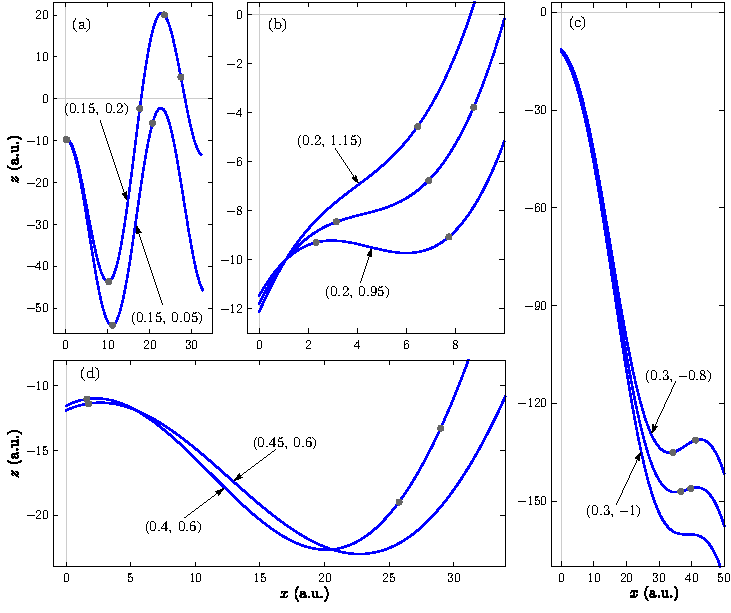
\includegraphics[scale=1]{5-Quantum-orbits/Figures/figure5H.pdf}
\end{center}   
  \caption[
  Classical trajectories near the critical points of the closest-approach surface
  ]{
  Classical trajectories from near the critical points marked \texttt{a}-\texttt{d} in \reffig{f5-classical-tca-plots}, where the closest-approach roots of \eqref{e5-tca-classical-equation} can merge and disappear, indexed by their reduced momentum $(\omega p_x/F,\omega p_z/F)$. The dots show closest-approach points, which satisfy \eqref{e5-tca-classical-equation} and for which the tangent to the trajectory is orthogonal to the radius vector.
  In the neighbourhood of a soft recollision, \protect\subref{f5-sample-trajectories-a}, an inward turning point turns into an outward turning point flanked by closest-approach points as the momentum increases.
  In \protect\subref{f5-sample-trajectories-b} and \protect\subref{f5-sample-trajectories-c} two turning points, a maximum and a minimum of $\rcl(t)^2$, merge and disappear as $p_z$ goes past the oscillation amplitude $F/\omega$, either in the positive \protect\subref{f5-sample-trajectories-b} or negative \protect\subref{f5-sample-trajectories-c} direction, so $v_z$ no longer changes sign and no turning points occur.
  Similarly, as the transverse momentum $p_x$ increases in \protect\subref{f5-sample-trajectories-d} the $x$ component of the velocity becomes too great for the tangent to be orthogonal to the radius vector; at that point a maximum and minimum of $\rcl(t)^2$ merge and disappear, leaving $\rcl(t)^2$ to grow monotonically.
  }
  \label{f5-sample-trajectories}
\end{figure}


The closest-approach solutions of \eqref{e5-tca-classical-equation} become more interesting when one allows a nonzero transverse momentum $\pt=p_x$. Here the solutions form a single coherent surface, shown in \ref{f5-classical-tca-surface}, that consists of a number of bounded lobes joined together at the soft recollisions, which locally look like cones. Thus, it is possible to continuously connect any two roots of~\eqref{e5-tca-classical-equation} via a path on the surface: the inward turning points and the recollisions, shown as separate green curves in \reffig{f5-classical-tca-on-axis}, can always be smoothly connected via the $p_x\neq 0$ component of the surface. This, in turn, precludes the existence of a simple criterion to distinguish one from the other in the general case.







\begin{figure}[t!]
  \centering
  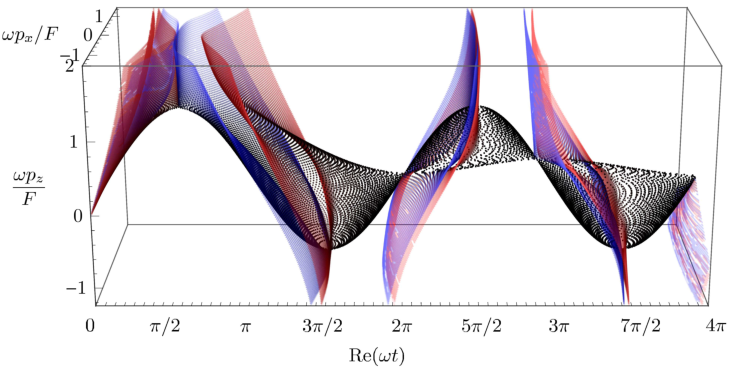
\includegraphics[scale=1]{5-Quantum-orbits/Figures/figure5I.pdf}
  \caption[
  Quantum solutions of the closest-approach equation
  ]{
  The quantum solutions of the closest-approach equation \eqref{e5-tca-equation} form multiple surfaces which wrap around the classical solutions of \reffig{f5-classical-tca-surface}, closely following the lobes, where the latter exist, and departing at the edges to form pairs of parallel surfaces with imaginary parts of opposite sign. 
  Black dots represent largely real solutions, with red (blue) dots representing solutions with positive (negative) imaginary part.
  An interactive 3D version of this figure is available as Fig.~\href{https://electrondynamicsincomplextimeandspace.github.io/\#figure-s2}{S2} in the Supplementary Information~\cite{SupplementaryInformation}.
 }
  \label{f5-quantum-tca-surface}
\end{figure}


On the other hand, the outward turning points can still be distinguished, as they are the local maxima of $\rcl(t)^2$ and have a different sign of the second derivative $\tfrac{\d^2}{\d t^2}\rcl(t)^2$. These maxima are shown in red in Figs.~\ref{f5-classical-tca-on-axis} and~\subref{f5-classical-tca-surface}, and they form the ``left-facing'' side of the surface in \reffig{f5-classical-tca-surface}. Thus, any horizontal line of constant momentum must enter the surface through a maximum of $\rcl(t)^2$ (red) and leave it through a minimum (green), because the minima and maxima must alternate for any given trajectory. This means that the red (maximum) side of the surface points towards negative $t$, and the green (minimum) side points towards positive $t$. At the boundary between these two parts of the surface, a maximum and a minimum merge and disappear, and the trajectory will then behave as shown in Figs.~\ref{f5-sample-trajectories-b}, \subref{f5-sample-trajectories-c}, or \subref{f5-sample-trajectories-d}, depending on which direction the boundary is approached (i.e. towards positive $p_z$, negative $p_z$, or increasing $|p_x|$, respectively). Horizontal lines of constant momentum will be tangent to the surface at this boundary, and the corresponding trajectory will have a double root of~\eqref{e5-tca-classical-equation}.



\subsection{Quantum solutions}

The quantum solutions have a richer geometry, with an additional dimension -- imaginary time -- to be occupied. The immediate effect of this is to increase the number of available solutions: while in the classical case two real solutions of~\eqref{e5-tca-classical-equation} can merge and disappear, as they do in the points marked \texttt{b} and \texttt{c} in \reffig{f5-classical-tca-on-axis}, in the quantum case the complex solutions of \eqref{e5-tca-equation} are not lost, but will instead move into imaginary time and remain present.



In general, the quantum solutions will be close to the classical ones when the latter exist. As one approaches the end of a lobe on the classical solution surface of \reffig{f5-classical-tca-surface}, however, the quantum solutions approach each other close to the real axis and then diverge into positive and negative imaginary time, keeping a relatively constant real part. If one then projects this to real times, the result is a pair of surfaces which closely follow the red and green parts of the classical surface, and then diverge into roughly parallel planes as they reach the end of each lobe. We show this behaviour in \reffig{f5-quantum-tca-surface}.


The first few closest-approach solutions are relatively easy to handle, and depend smoothly on the momentum. This includes the first minimum and maximum of $\rl(t)^2$, like the ones in \reffig{f5-complex-position-contour-plot}, the birth time $\ts$ itself, and a conjugate solution with negative imaginary part which should be ignored. These solutions occupy specific regions of the complex $t$ plane, as shown in \reffig{f5-complex-tca-plane-structures}, and they can be identified consistently. Moreover, these solutions exhibit close approaches at $\omega t\approx \pi/2$ and $\omega t \approx 3\pi/2$, which are the quantum counterpart of the classical maximum-minimum mergers shown in Figs.~\ref{f5-sample-trajectories-b} and~\subref{f5-sample-trajectories-c}. These are evident in \reffig{f5-complex-tca-plane-structures} as the converging surfaces at those times, and they are of relatively limited interest.



\begin{figure}[t!]
  \centering
  \begin{tabular}{c}
  \subfloat{
    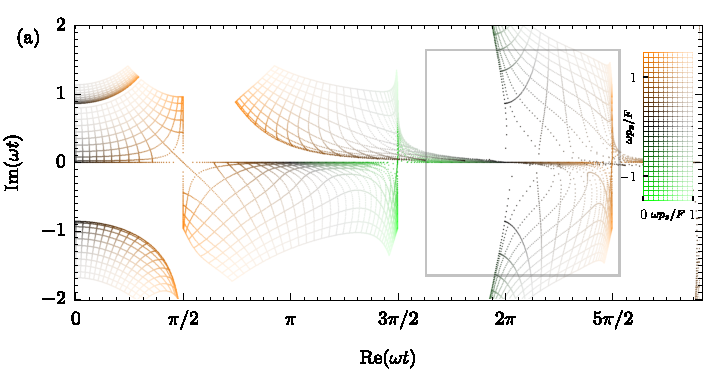
\includegraphics[scale=1]{5-Quantum-orbits/Figures/figure5Ja.pdf}
    \label{f5-tca-grid-patterns}
  }
  \\[-3mm]
  \begin{tabular}{cc}
  \subfloat{
    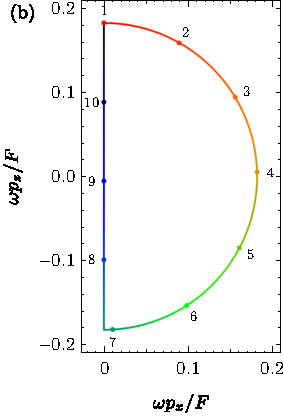
\includegraphics[scale=1]{5-Quantum-orbits/Figures/figure5Jb.pdf}
    \label{f5-momentum-semicircle}
  }
  &
  \subfloat{
    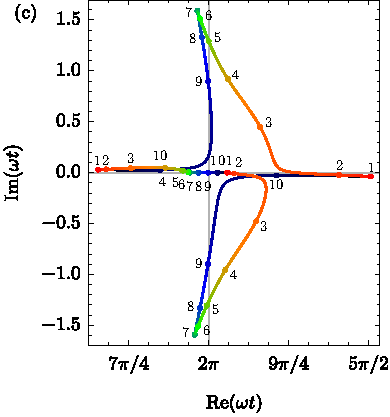
\includegraphics[scale=1]{5-Quantum-orbits/Figures/figure5Jc.pdf}
    \label{f5-tca-mixing-paths}
  }
  \end{tabular}
  \end{tabular}
  \caption[
  Quantum closest-approach times on the complex time plane
  ]{
  The quantum closest-approach times, which satisfy \eqref{e5-tca-equation}, on the complex time plane. In \protect\subref{f5-tca-grid-patterns} we show the closest approach times corresponding to a grid in momentum space (shown inset). These are generally grid-like in the time plane, though after $\omega t=3\pi/2$ some solutions lie close to the real axis and cannot be discerned in this view.
  At the cusps of Figs.~\ref{f5-classical-tca-surface} and \ref{f5-quantum-tca-surface}, which correspond to soft recollisions, the regular grid-like behaviour breaks and the solutions can no longer be uniquely tagged. 
  This can be seen by following the semicircular path in momentum space shown in \protect\subref{f5-momentum-semicircle}, for which there are three solutions in the gray rectangle of \protect\subref{f5-tca-grid-patterns}, shown in detail in \protect\subref{f5-tca-mixing-paths}. Going once around the semicircle moves the $\tca$ along the bow-shaped curves and, upon returning to the initial point, permutes them cyclically.
  In particular, this path contains an avoided collision between the points marked 2 and 3, and a three-way avoided collision between points 9 and 10. This three-way interaction marks the soft recollision itself.
  An interactive 3D version of this figure, with considerable additional detail, is available as Figs.~\href{https://electrondynamicsincomplextimeandspace.github.io/\#figure-s3}{S3} and~\href{https://electrondynamicsincomplextimeandspace.github.io/\#figure-s4}{S4} in the Supplementary Information \cite{SupplementaryInformation}.
 }
  \label{f5-complex-tca-plane-structures}
\end{figure}


%\begin{figure}
%\caption{hello, this is a \href{http://google.com\#hello}{test}}
%\end{figure}



The most important $\tca$ close approaches occur at and near the soft recollisions, shown inside the gray rectangle of \reffig{f5-tca-grid-patterns} and in \reffig{f5-tca-mixing-paths}, with a complicated momentum dependence which we explore below. In the quantum domain, soft recollisions again represent interactions between three different closest-approach roots. Unlike the classical domain, however, the roots do not merge; instead, two of them move into imaginary time after a three-way avoided collision, shown in \reffig{f5-tca-mixing-paths} between the points marked 9 and~10. The proximity between the multiple saddle points mirrors the increased time the electron spends near the ion in the neighbourhood of a soft recollision.

More interestingly, this three-way collision marks a crucial topological change in the configuration of the branch cuts associated with the recollision, as shown in \reffig{f5-branch-cut-topology-change}. Each of the outer saddle points, $\tcasup{\,(1)}$ and $\tcasup{\,(3)}$, has a pair of branch cuts associated with it, in the same `slalom gate' configuration as in \reffig{f5-tCA-zoom}, and these go off into imaginary time. However, the way in which they do so changes as the longitudinal momentum $p_z$ passes the momentum $\pzsr$ of the soft recollision.


For $p_z$ below $\pzsr$, as in \reffig{f5-branch-cut-topology-open}, the branch cuts loop back to imaginary time without crossing the real time axis. As with the low-momentum trajectory of \reffig{f5-sample-trajectories-a}, the trajectory does not quite reach the collision, and the associated branch cuts do not force a change of contour. At $p_z=\pzsr$, however, the branch cuts touch and reconnect, and for $p_z>\pzsr$ the topology changes to the one shown in \reffig{f5-branch-cut-topology-closed}. Here the trajectory does pass the core, and the associated branch cuts do cross the real axis, forcing the integration contour to change and pass through the gates.


This process has profound implications for the ionization amplitude, because these drastic changes in the integrand occur precisely when it is largest. Thus, choosing the wrong contour in this region accounts for the largest contributions to the integrand, with a correspondingly large effect on the integral. More surprisingly, once the contour is forced to pass through the `gate' $\tca$s, for $p_z$ just above $\pzsr$, their contributions have the effect of suppressing the ionization amplitude there. We will see how this works in more detail in chapter~\ref{chap:LES-NZES}.


We now turn to the momentum dependence of the closest-approach times near the soft recollision, which again presents interesting topological features. The main problem is illustrated in Figs.~\ref{f5-momentum-semicircle} and \subref{f5-tca-mixing-paths}: the different solutions of \eqref{e5-tca-equation} mix, and there is no longer any way to distinguish them from each other, as there was in the classical case. More concretely, traversing a closed loop in momentum space, like the semicircle shown in \reffig{f5-momentum-semicircle}, will move the roots around in such a way that when one returns to the initial point the overall configuration is the same, but the saddle points have been permuted cyclically.

Topologically, this means that the surface defined by \eqref{e5-tca-equation} (a two-dimensional surface in a four-dimensional space) does not separate into distinct components; instead, the surface has a single connected component after $\omega t=3\pi/2$. On the other hand, the surface itself remains singly connected. 
%
%Both of these behaviours are explored in Figs.~S3 and S4 in the Supplementary Information~\cite{SupplementaryInformation}.


This mixing behaviour is unusual in the quantum orbit formalism, where the norm is for rather elaborate indexing schemes to be possible \cite{Becker_rescattering, milosevic_ISFA-standard_2007}, partly because there is usually a single free parameter that governs the motion of the saddle points. Here the control space is two-dimensional, which allows for nontrivial closed loops inside it, and this defeats the possibility of attaching any type of label to individual roots of~\eqref{e5-tca-equation}. 


To be more explicit, it would be convenient to have an alphabet $\mathcal A$ (i.e. a set of discrete labels to tag the roots with, analogous to the set $\{(\alpha,\beta, m)\}$ of Refs.~\citealp{Becker_rescattering, milosevic_ISFA-standard_2007}), together with a tagging function $A\colon \mathcal S \to \mathcal A$ that takes the solution set
\begin{equation}
\mathcal S = \left\{ (\vbp,\tca)\in\mathbb{R}^3\times\mathbb{C}  
\mathrel{}\middle|\mathrel{}
(\vbp+\vba(\tca))\cdot\int_{\ts}^{\tca} (\vbp+\vba(t))\d t=0 
%\text{ for some } \vbp\in\mathbb{R}^3 
\right\}
\end{equation}
of all closest-approach times and assigns each momentum and $\tca$ a label $A(\vbp,\tca) \in \mathcal A$ in a continuous way, and such that for each label $a\in\mathcal A$ the preimage $A^{-1}(a)\subset \mathcal S$ contains a unique root for each momentum $\vbp$. Unfortunately, the existence of nontrivial loops like the one in 
Figs.~\ref{f5-momentum-semicircle} and \subref{f5-tca-mixing-paths} means that any such mapping must either be discontinuous (at locations which must therefore be arbitrary) or assign a single label to all the roots of \eqref{e5-tca-equation} after $\Re(\tca)>3\pi/2$. 


Finally, an interesting consequence of the mixing between roots is that, at certain specific values of $p_x$ and $p_z$, the roots must merge, giving double roots of~\eqref{e5-tca-equation}. However, this behaviour depends very sensitively on the momentum, and it can safely be ignored. (In fact, the very difficulty of tagging the roots, caused by the mixing, makes finding the merge momentum an elusive numerical problem.)


\section{Navigating the branch cuts}
We have seen, then, that it is possible, given any pair of branch cuts, to consistently find a point $\tca$ that sits between them and guarantees a safe passage between the cuts for an integration path. However, these points are found as the solutions of an equation that yields several other roots, and in general it is impossible to distinguish the different types~of~roots. 


Moreover, as shown for example in \reffig{f5-branch-cut-sketch-open}, it can be actively harmful to pass through some of these roots: not all the $\tca$ are useful stepping stones, so in addition to having a way to find the set of stepping stones, we also require a way to choose which $\tca$s the path should go through, and in what order.

This certainly appears as a difficult problem, because such an algorithm should know to reject $\tcasup{\,(1)}$ and $\tcasup{\,(3)}$ in \reffig{f5-branch-cut-sketch-open}, but to take the integration path through them in \reffig{f5-branch-cut-sketch-closed}, even though locally the surface of $\sqrt{\rl(t)^2}$ at each of them is essentially identical, and the two are very close together in momentum space. 

Fortunately, though, it is indeed possible to algorithmically distinguish between the two cases, based on the geometrical fact shown in Figs.~\ref{f5-branch-cut-velocity-open} and \subref{f5-branch-cut-velocity-closed}: the topological change in the structure of the branch cuts between \reffig{f5-branch-cut-sketch-open} and \reffig{f5-branch-cut-sketch-closed} happens simultaneously with a change in the sign of the real part of the squared velocity, $\Re(\vbv(\tcasup{\,(j)})^2)$, of the outer saddle points. Thus, in the closed topology of \reffig{f5-branch-cut-sketch-closed}, where the integration path should pass through all of the $\tcasup{\,(j)}$, the real part of the kinetic energy is positive at those saddle points, whereas in the open topology of \reffig{f5-branch-cut-sketch-open}, where the path  should ignore the outer roots, $\Re(\vbv(\tcasup{\,(1)})^2)$ and $\Re(\vbv(\tcasup{\,(3)})^2)$ are both negative.

The physical content of this criterion is quite clear: in the quantum-orbit formalism, the classically forbidden regions are readily identified in the complex time plane as those regions where the kinetic energy $\frac12 \vbv(t)^2$, or at least its real part, is negative. The undesirable saddle points of \reffig{f5-branch-cut-sketch-open} therefore require the trajectory to tunnel towards the core to be reached, and this is clearly unwanted on physical grounds.

On the other hand, a formal proof of the simultaneity of the topological change in the branch cut structure with the emergence of the $\tca$ from the `barrier' region where~$\Re(\vbv(\tca)^2)<0$ is still lacking; indeed, it appears rather challenging to relate the two structures, since one is a global topological measure and the other is a local measure of a different, only distantly related, dynamical quantity. Thus, at present, this is an empirical fact, with a formal proof left as an interesting open question of the mathematical aspects of this work.







\newgeometry{left=18mm,right=18mm,bottom=10mm}


\captionsetup[figure]{position=top}

\newcommand{\figurefiveKscale}{1}
\begin{figure}[p]
\centering
  \begin{tabular}{cc}
  $\qquad p_z=\figurefiveKppl{}F/\omega$   &    $p_z=\figurefiveKpph{}F/\omega$  
  \\  \hline  \vspace{-2mm} \\
  \subfloat[$\sqrt{\rl(t)^2}$\hspace{-6pt}$\,$]{
    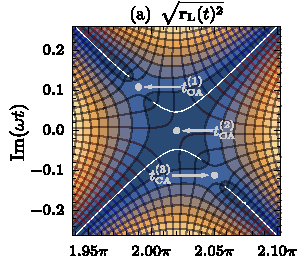
\includegraphics[scale=\figurefiveKscale]{5-Quantum-orbits/Figures/figure5Ka.pdf}
    \label{f5-branch-cut-topology-open}
  }
  & \hspace{-6mm}
  \subfloat[$\sqrt{\rl(t)^2}$ \hspace{10mm}$\,$]{
    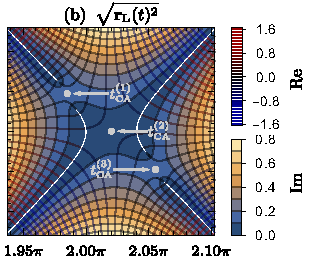
\includegraphics[scale=\figurefiveKscale]{5-Quantum-orbits/Figures/figure5Kb.pdf}
    \label{f5-branch-cut-topology-closed}
  }
  \\
  \subfloat[$\vbv(t)^2$]{
    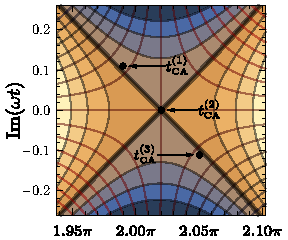
\includegraphics[scale=\figurefiveKscale]{5-Quantum-orbits/Figures/figure5Kc.pdf}
    \label{f5-branch-cut-velocity-open}
  }
  & \hspace{-6mm}
  \subfloat[$\vbv(t)^2$\hspace{10mm}$\,$]{
    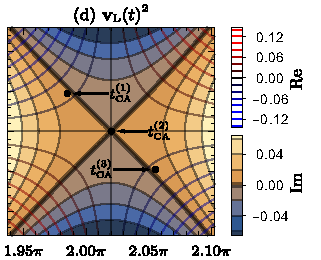
\includegraphics[scale=\figurefiveKscale]{5-Quantum-orbits/Figures/figure5Kd.pdf}
    \label{f5-branch-cut-velocity-closed}
  }
  \\
  \subfloat[Branch cut sketch]{
    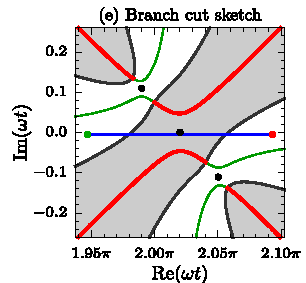
\includegraphics[scale=\figurefiveKscale]{5-Quantum-orbits/Figures/figure5Ke.pdf}
    \label{f5-branch-cut-sketch-open}
  }
  & \hspace{-6mm}
  \subfloat[Branch cut sketch\hspace{15mm}$\,$]{
    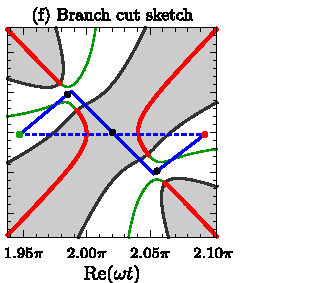
\includegraphics[scale=\figurefiveKscale]{5-Quantum-orbits/Figures/figure5Kf.pdf}
    \label{f5-branch-cut-sketch-closed}
  }
  \end{tabular}

  \begin{tabular}{cc}
  \subfloat[Trajectory]{
    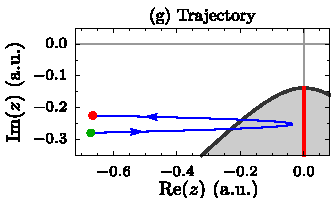
\includegraphics[scale=\figurefiveKscale]{5-Quantum-orbits/Figures/figure5Kg.pdf}
    \label{f5-branch-cut-trajectory-open}
  }
  & \hspace{-6mm}
  \subfloat[Trajectory]{
    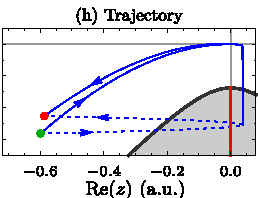
\includegraphics[scale=\figurefiveKscale]{5-Quantum-orbits/Figures/figure5Kh.pdf}
    \label{f5-branch-cut-trajectory-closed}
  }
  \end{tabular}
  \captionsetup{width=\textwidth}
  \caption[
  Topological transition, with a branch cut reconnection, at the soft recollision, coinciding with the emergence of the closest-approach times from the tunnelling barrier
  ]{
    During a soft recollision, the quantum times of closest approach will perform a three-way close approach, like that shown in Fig. \ref{f5-tca-mixing-paths} at the first soft recollision between the points 9 and 10. At this close approach, the branch cuts associated with these saddle points will reconnect and change topologies, as shown in \protect\subref{f5-branch-cut-topology-open} and \protect\subref{f5-branch-cut-topology-closed} (and sketched in \protect\subref{f5-branch-cut-sketch-open} and \protect\subref{f5-branch-cut-sketch-closed}, as in \reffig{f5-branch-cut-sketch}). 
    At the point of the topological change, the outer saddlepoints $\tcasup{\,(1)}$ and $\tcasup{\,(3)}$ emerge from the classically forbidden region, and the real part of their kinetic energy $\Re(\tfrac12\vbv(t)^2)$ changes sign, as shown in \protect\subref{f5-branch-cut-velocity-open} and \protect\subref{f5-branch-cut-velocity-closed}. 
%    After the change, the outer saddlepoints do not require tunnelling to get to, and should be crossed by the integration contour.
%    We show in \protect\subref{f5-branch-cut-sketch-open} and \protect\subref{f5-branch-cut-sketch-closed} a sketch of the relevant branch cuts, analogous to \reffig{f5-branch-cut-sketch}, along with the appropriate integration contour for each topology.
    In \protect\subref{f5-branch-cut-trajectory-open} and \protect\subref{f5-branch-cut-trajectory-closed} we show the corresponding trajectories in the complex $z$ plane for those contours. The motion along $z$ is similar to \reffig{f5-sample-trajectories-a}, with a modest imaginary part as in \reffig{f5-imaginary-parts-of-position}, and if the core is not reached does not represent a problem. For the slightly higher momentum of~\protect\subref{f5-branch-cut-trajectory-closed}, however, the trajectory passes the origin and would cross the associated branch cut if taken along the dashed integration contour of \protect\subref{f5-branch-cut-sketch-closed}, so the contour must be deformed to avoid it, as shown by the solid line.
    Here~$p_x=\figurefiveKpo$.
}
\label{f5-branch-cut-topology-change}
\end{figure}


\captionsetup[figure]{position=auto}

\restoregeometry
\clearpage
\onehalfspacing










On the other hand, a formal proof of the simultaneity of the topological change in the branch cut structure with the emergence of the $\tca$ from the `barrier' region where~$\Re(\vbv(\tca)^2)<0$ is still lacking; indeed, it appears rather challenging to relate the two structures, since one is a global topological measure and the other is a local measure of a different, only distantly related, dynamical quantity. Thus, at present, this is an empirical fact, with a formal proof left as an interesting open question of the mathematical aspects of this work.



With this final piece in place, we can set some definite rules for how to choose a contour path. In general, it is sufficient to take, in order of increasing $\Re(\tca)$, those closest-approach times which (i) occur after ionization, (ii) have a reasonably bounded imaginary part, and (iii) have positive kinetic energy. 

To this we add two exceptions. First, we always include the first inward turning point, which lies in the half-strip $-\pi/2<\Re(\omega t)<\pi/2$, $\Im(t)>0$ (as exemplified in \reffig{f5-tca-grid-patterns}) and which helps the integration path avoid regions where $\Re(\vbv(t)^2)<0$ and there is no need to cross them. Secondly, we always include the first closest-approach time, in the strip $\pi/2<\Re(\omega t)<3\pi/2$, $\Im(t)>0$, where it can always be consistently identified, is always necessary to keep the contour on track, and can in some cases have an imaginary part larger than the ionization time.

Putting all of this together, the concrete set of rules we use for choosing the contour is to take those $\tca$s for which
\begin{enumerate}[itemsep=-0.8mm]
\item[] $\Re(\omega \tca)>\omega\tn +\pi/5$ \textbf{and}
\item[] $-\frac13 \tauT<\Im(\tca)\leq \Im(\tk)$ \textbf{and}
\item[] $\Re\left(\vbv(\tca)^2\right) > -u$,
\item[\textbf{or}\hspace{3pt}] $-\pi/2 < \Re(\omega\tca) < \pi/2$ \textbf{and}
\item[] $0\leq\Im(\tca)<\tauT$,
\item[\textbf{or}\hspace{3pt}] $\pi/2 < \Re(\omega\tca) < 3\pi/2$ \textbf{and}
\item[] $\Im(\tca)>0$,
\end{enumerate}
and then traverse them in order of increasing $\Re(\tca)$. (Here $u$ is an adjustable numerical precision, for additional flexibility with the precise moment of emergence of the $\tca$s from the `barrier', which we set by default to $\SI{e-8}{\au}$)

%%% Note hackish \au - period interaction above.


\captionsetup[figure]{position=top}

\newlength{\figurefiveLwidth}
\setlength{\figurefiveLwidth}{0.60\columnwidth}
\begin{figure}[t!]
  \centering
  \begin{tabular}{c}
    \subfloat[$\vbp=(\figurefiveLapo,0,\figurefiveLapp)$]{
      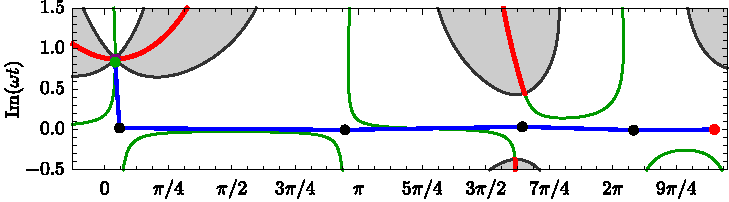
\includegraphics[scale=1]{5-Quantum-orbits/Figures/figure5La.pdf}  
      \label{f5-path-chooser-examples-a}
    }
    \\
    \subfloat[$\vbp=(\figurefiveLbpo,0,\figurefiveLbpp)$]{
      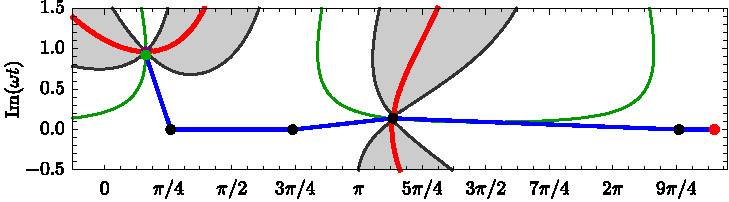
\includegraphics[scale=1]{5-Quantum-orbits/Figures/figure5Lb.pdf}  
      \label{f5-path-chooser-examples-b}
    }
    \\
    \subfloat[$\vbp=(\figurefiveLcpo,0,\figurefiveLcpp)$]{
      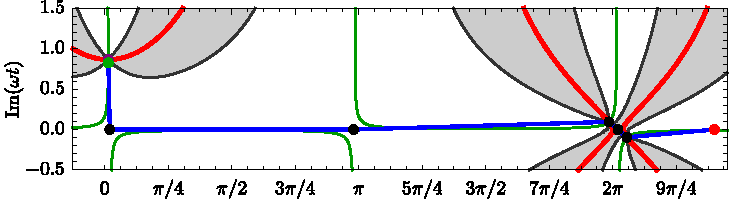
\includegraphics[scale=1]{5-Quantum-orbits/Figures/figure5Lc.pdf}  
      \label{f5-path-chooser-examples-c}
    }
    \\
    \subfloat[$\vbp=(\figurefiveLdpo,0,\figurefiveLdpp)$]{
      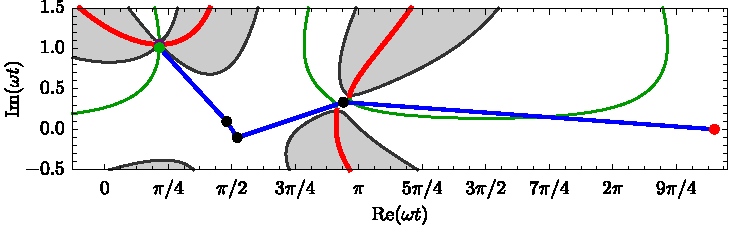
\includegraphics[scale=1]{5-Quantum-orbits/Figures/figure5Ld.pdf}  
      \label{f5-path-chooser-examples-d}
    }
  \end{tabular}
  \captionsetup{width=\textwidth}
  \caption[
  Sample integration paths produced by the $\tca$ choosing algorithm 
  ]{
  Sample integration paths produced by the $\tca$ choosing algorithm described in the text. Most momenta are straightforward \protect\subref{f5-path-chooser-examples-a}, but near-recollision momenta, like the one shown in \reffig{f5-complex-position-branch-cuts}, do require careful handling, as shown in \protect\subref{f5-path-chooser-examples-b}. The algorithm correctly handles soft recollisions, \protect\subref{f5-path-chooser-examples-c}, as well as higher momenta with harder recollisions~\protect\subref{f5-path-chooser-examples-d}.
  }
  \label{f5-path-chooser-examples}
\end{figure}


\captionsetup[figure]{position=auto}



These rules are relatively heuristic, and they have a fair amount of leeway around them in the choice of parameters. (For example, the choice of $-\frac13 \tauT$ as a lower bound for $\Im(\tca)$ is not particularly strict, and it serves mostly to rule out the extraneous conjugate solution at $\Im(t)<0$, $-\pi/2<\omega t<\pi/2$ shown in \reffig{f5-tca-grid-patterns}.) However, they work well over the relevant region of photoelectron momenta to produce correct integration path choices, particularly including the delicate changes required near soft recollisions as exemplified in \reffig{f5-branch-cut-topology-change}, so they are good enough for the job. (Nevertheless, when using such contours it is always necessary to use a numerical integration algorithm that can detect when the integrand has a discontinuity, and if any such errors are reported during integration they should be duly investigated.)





We display in \reffig{f5-path-chooser-examples} some sample integration contours produced (automatically) with this criterion, which is implemented in software in \citer{ARMSupport}. In general, the navigation is relatively straightforward, and there are never any problems when $p_z<0$ or $\pt$ is sizeable, in which case the contour looks as in \reffig{f5-path-chooser-examples-a}. For electrons that get closer to the nucleus during their oscillations, however, the branch cuts do require more careful navigation, as we have seen, and this is still handled well, as shown in \reffig{f5-path-chooser-examples-d}.


Another feature to note is that in some very specific cases, very close to a soft recollision as shown in \reffig{f5-branch-cut-topology-change} and particularly \reffig{f5-branch-cut-sketch-closed}, the integration path chosen by the above algorithm is topologically correct, but it may pass very close to a Coulomb singularity. While this is formally not a problem, it is not conceptually ideal, so there is some room for improvement in future work if it becomes necessary.


In addition, it is important to note from Figs.~\ref{f5-branch-cut-sketch-open} and \subref{f5-branch-cut-sketch-closed} that at certain momenta, very close to the soft recollision, the gray areas where $\Re(\rl(t)^2)<0$ that surround the branch cuts can join up, creating a passage where all the possible integration paths must necessarily have parts where $\Re(\rl(t)^2)<0$. As far as the Coulomb potential goes, this is not really a problem, because the branch cuts have been correctly handled, but this is also the region where we can no longer trust any correlation interaction potentials obtained through numerical, quantum chemical calculations, as we saw in chapter~\ref{chap:complex-space-potentials}. Fortunately, this region is very small, and as we shall see in the following chapter the dynamics of the photoelectron yield are dominated by the Coulomb dynamics of the direct term, so the correlation-driven yield can safely be ignored in that range.




































   
